\chapter{Background}

\par Oridinarily, real-world data contains 3-dimensions. 
Because standard images only include 2-dimensional data, information regarding depth is lost (i.e. it is often difficult to judge distance from a single image without visual cues). 
\textit{Stereovision} attempts to resolved this by finding the same point in both \textit{stereoscopic} images (known as a \textit{corresponding point}), and recovering the depth information.
An elementry example of this occurs in stereoscopic images with relatively low distance between cameras (i.e they are righht next to each other). 
Objects that are \textit{farther} away from the observer occur closer together in the stereo images, whereas objects \textit{closer} to the camera appear appear farther appart in the stereo-images.

\section{Change of Reference}

\par Each view from a pair of stereo-images encompasses its own \textit{frame of reference} (i.e. the directions of \textit{forward} or \textit{backward} are unique to image and may differe considerably depending on camera displacement).
This requires expressing points from different frames of reference (traditionally referred to \textit{left} and \textit{right}) in a single reference frame. 
As such it is necessary to be able to express coordinates in a given reference frame in any other reference frame.

\par Coordinates given in $\xR$ can be expressed in $\xL$ by the geometric transformation:
%\renewcommand{\arraystretch}{1.5}
\par
\begin{align*}
	\xL = \rLR \cdot \xR + \rLt
\end{align*}
or
\begin{align*}
	\hxL &=
	\left[\begin{array}{c|c}
		\rL\textbf{R} & \rL\textbf{t} \\\hline
		0 & 1 \\
	\end{array}\right]
	\cdot\hxR \\
	&\\
	&= \rLM\cdot\hxR\\
\end{align*}
where $\rLM$ is also the geometric transformation necessary to transform $\sL$ into $\sR$. 

\par Withough calculating any new quantities, rearranging allows us to express coordinates in $\xL$ in the $\xR$ reference frame as:

\par \begin{equation*}
	{\rLR\tT}\cdot (\xL - \rLt ) = \xR
\end{equation*}
and similarly transforms $\sR$ into $\sL$.

\section{Points and Lines in the Image Plane}

\par Points in \textit{world-space} of $\mathbb{R}^3$ are converted to points in the \textit{image-plane} of $\mathbb{R}^2$ by \textit{homogenization}. This occurs when a \textit{world-coordinate} of $\mathbf{x}=[x_1,x_2,x_3]^\intercal$ is mapped to a \textit{homogeneous image coordinate} of $\mathbf{\tilde{y}}=[y_1,y_2,1]^\intercal=[x_1/x_3,\;x_2/x_3,\;x_3/x_3]^\intercal$ or a \textit{non-homogeneous image coordinate} of $\mathbf{y}=[y_1,y_2]^\intercal=[x_1/x_3,\;x_2/x_3]^\intercal$. Points of the form $\mathbf{\tilde{y}}=[y_1,y_2,0]^\intercal$ are special case of homogeneous point referred to as a \textit{point at infinity}.

\par Lines in $\mathbb{R}^2$ can be represented in different contexts. The \textit{vector offset} method calculates a line $\mathbf{s}(t)$ between points $\mathbf{y_1}$ and $\mathbf{y_2}$ as 
%$\mathbf{s}(t)=(1-t)\cdot\mathbf{y_1}+t\cdot\mathbf{y_2}=\mathbf{y_1}+t\cdot(\mathbf{y_2}-\mathbf{y_1})$
\begin{equation*}
\begin{split}
\mathbf{s}(t)&=(1-t)\cdot\mathbf{y_1}+t\cdot\mathbf{y_2}\\
&=\mathbf{y_1}+t\cdot(\mathbf{y_2}-\mathbf{y_1})\\
\end{split}
\end{equation*}
in which the line is parrallel to the vector $\mathbf{y_2}-\mathbf{y_1}$ and offset from the  origin by the vector $\mathbf{y_1}$. Lines are also represented by their coefficients as $\mathbf{l}=[a,b,c]^\intercal$ where
\begin{equation*}
\begin{split}
\mathbf{l}^\intercal\cdot\mathbf{\tilde{y}}&=\left[\begin{array}{ccc}a & b & c\end{array}\right]\cdot\left[\begin{array}{c}y_1\\y_2\\1\end{array}\right]\\
&=a\cdot{y_1}+b\cdot{y_2}+c\cdot{1}\\
&=0
\end{split}
\end{equation*}
This definition lets us say $\mathbf{\tilde{y}}$ is located on line $\mathbf{l}$ \textit{if and only if} $\mathbf{l}^\intercal\cdot\mathbf{\tilde{y}}=0$. The line $\mathbf{l}$ joining two \textit{homogeneous image coordinates} $\mathbf{\tilde{y}_1}$ and $\mathbf{\tilde{y}_2}$ is then calculated as the cross product of $\mathbf{l}=\mathbf{\tilde{y}_1}\times\mathbf{\tilde{y}_2}$. 

\section{Epipolar Geometry}

\par Each point of of interest (also referred to as a \textit{feature}) in a single image occurs in a 2-dimensional space at location $\mathbf{\tilde{y}}=[x,y,1]^\intercal$. The same point in space when viewed from an image at a similar (though different) angle is referred to as a \textit{corresponding point} with location of $\mathbf{\tilde{y}'}=[x',y',1]^\intercal$\footnote{A \textit{change of reference} is implied between cooridinates $\mathbf{\tilde{y}}=[x', y', 1]^\intercal$ and $\mathbf{\tilde{y}'}=[x', y', 1]^\intercal$. The majority of corresponding points do not occur at the same \textit{image coordinates} between images (i.e $\mathbf{\tilde{y}}\neq\mathbf{\tilde{y}'}$. The only way a single \textit{world coordinate} can yield different \textit{image coordinates}, is if a \textit{change of reference} occurs in \textit{world space} each time the \textit{image coordinates} are obtained by dividing by $z_{world}$.}. This set of infinitley many points form a 1-dimensional subspace (also known as a \textit{pencil}) of the 3-dimensional world space.

\par The pencil, when viewed from an image at a different angled-position, appears as a line $\mathbf{l'}=[A',B',C']^\intercal$, known as the \textit{epipolar line}. The fact that the corresponding point (in the \textit{angled image}) of $\mathbf{\tilde{y}'}=[x',y',1]^\intercal$ occurs on this epipolar line is referred to as the \textit{epipolar constraint}. It is formalized, using the previously given \textit{line-point equality} of $\mathbf{l'}^\intercal\cdot\mathbf{\tilde{y}'}=0$ for the \textit{angled} image. Similarly, the corresponding point of $\mathbf{\tilde{y}'}=[x',y',1]^\intercal$ produces an epipolar line in the \textit{original image} of $\mathbf{l}=[A,B,C]$. The original point of $\mathbf{\tilde{y}}=[x,y,1]^\intercal$ must lie located on this epipolar line as required by the epipolar constraint, resulting in the \textit{line-point equality} of $\mathbf{l}^\intercal\cdot\mathbf{\tilde{y}}=0$ for the \textit{original image}. 

\par When viewed in ther respective images, each point ($\mathbf{\tilde{y}}$ and $\mathbf{\tilde{y}'}$) has a pencil that coincides with that point. Since the pencils act as \textit{directional}-vectors in 3-dimensional space, there is a unique 2-dimensional plane which contain both of these vectors, known as the \textit{epipolar plane}. It is the intersection of the epipolar plane with the \textit{original image}-plane and the \textit{angled image}-plane that results in the epipolar lines of $\mathbf{l}$ and $\mathbf{l'}$, respectively. In fact, the \textit{epipolar plane} (in each image's \textit{coordinate systems})\footnote{There is a single \textit{epipolar plane} for each pair of corresponding points $\mathbf{\tilde{y}}$ and $\mathbf{\tilde{y}'}$. However, the single plane can be parameterized infinitley many ways, depending on the \textit{frame of reference}} has the same vector form as its epipolar line. Specifically, in the \textit{original image} reference frame $\mathbf{l}=\mathbf{P}=[A,B,C]^\intercal$, and in the \textit{angled image} reference frame $\mathbf{l'}=\mathbf{P'}=[A',B',C']^\intercal$. This results from the fact that any \textit{world}-point $\mathbf{x}$ lying on the \textit{epipolar plane} $\mathbf{P}$ will result in a \textit{homogeneous image}-point $\mathbf{\tilde{y}}$ that also lies on the plane $\mathbf{P}$. Specifically, when $\mathbf{x}=s\cdot\mathbf{\tilde{y}}$ for some non-zero value of \textit{s}, then $\mathbf{P}^\intercal\cdot\mathbf{x}=0$ implies $\mathbf{P}^\intercal\cdot\mathbf{x}=\mathbf{P}^\intercal\cdot(s\cdot\mathbf{\tilde{y}})=0$. Since $s\neq0$, its true that $\mathbf{P}^\intercal\cdot\mathbf{\tilde{y}}=0$. 

\par In the majority of images, the sets of epipolar lines will converge at a point known as an \textit{epipole}, denoted as $\mathbf{e}$ in the \textit{original image} and $\mathbf{e'}$ in the \textit{angled image}. 

\section{Fundamental Matrix}
In stereo vision, points ($\mathbf{\tilde{x}}$) in one image $I$ are related to the epipolar line ($l'$) that contain the corresponding point ($\mathbf{\tilde{x}}'$) by the \textit{Fundamental Matrix} ($\mathbf{F}$).
\begin{equation*}
l'=\mathbf{F}\cdot\mathbf{\tilde{x}}
\end{equation*}

\section{Camera Calibration Matrix}

\subsection{Pinhole Camera Model}

\par A point $\mathbf{x}$ in the \textit{camera-coordinate system} of $\mathbb{R}^3$ is projected to the point $\mathbf{\tilde{y}}$ in $\mathbb{R}^{2}$ by means of the \textit{pinhole camera model}. The set of all $\mathbf{\tilde{y}}$ are the result of \textit{rays} passing through the \textit{image plane} located at $z=f$, and converging at the \textit{optical center} as shown in the figure below:
\begin{figure}[htbp]
	\centering
%	\includesvg{BiLinear_Point_Correspondance_v1}
	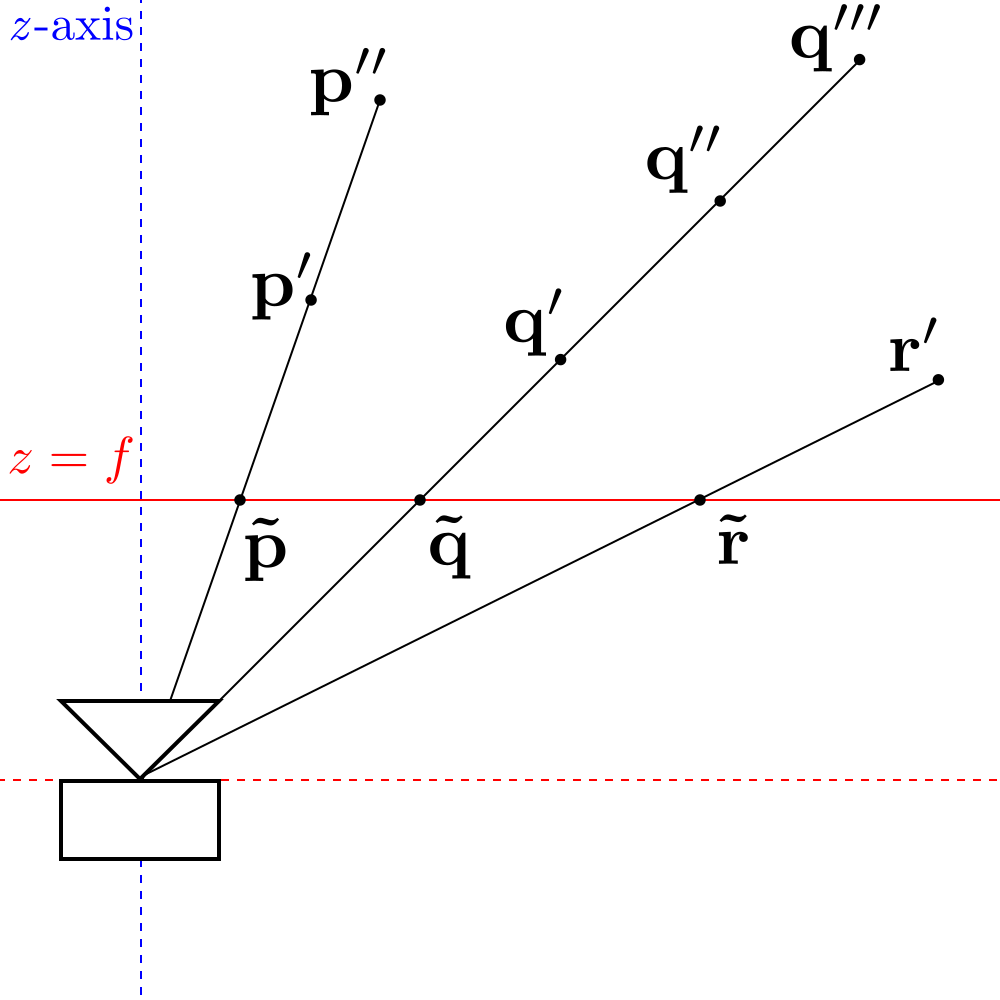
\includegraphics[scale=0.25]{Camera}
	\caption{Pinhole CameraModel}
\end{figure}\newline
The exact location that $\mathbf{\tilde{y}}$ appears on the image plane is determined by utilizing the \textit{similarity of triangles} between $\mathbf{x}$ and $\mathbf{\tilde{y}}$. 
Specifically, we see that $y_1/f=x_1/x_3$ and $y_2/f=x_2/x_3$ rearranged gives $x_3\cdot y_1=f\cdot x_1$ and $x_3\cdot y_2=f\cdot x_2$ . This lets us relate $\mathbf{\tilde{x}}$ and $\mathbf{\tilde{y}}$ by the \textit{projection matrix} $\mathbf{P}$ as

\begin{equation*}
\begin{split}
x_3\cdot\mathbf{\tilde{y}}
%=
%x_3\cdot\begin{bmatrix}y_1\\y_2\\1\end{bmatrix}
=
\mathbf{P}\cdot\mathbf{\tilde{x}}
=
\begin{bmatrix}
f & 0 & 0 & 0\\
0 & f & 0 & 0\\
0 & 0 & 1 & 0\\
\end{bmatrix}\cdot\begin{bmatrix}x_1\\x_2\\x_3\\1\end{bmatrix}
\end{split}
\end{equation*}%
Since, for a given $\mathbf{x}$ in \textit{camera space}, the quantities 
$x_{1/3}=x_1/x_3$ and $x_{2/3}=x_2/x_3$ 
%$x_1/x_3$ and $x_2/x_3$ 
are \textit{invariant under the scale of $\mathbf{x}$} 
%will be constant \textit{regardless of the units of $\mathbf{x}$}, 
the location of $\mathbf{\tilde{y}}$ in the \textit{image plane} depends only on the ratios $x_{1/3}$ and $x_{2/3}$ and the quantity $f$. This yields a similar form, obtained from dividing by $x_3$, of

\begin{equation*}
\begin{split}
\mathbf{\tilde{y}}
%=
%\begin{bmatrix}y_1\\y_2\\1\end{bmatrix}
=
\frac{1}{x_3}\mathbf{P}\cdot\mathbf{\tilde{x}}
=
\frac{1}{x_3}\begin{bmatrix}
f & 0 & 0 & 0\\
0 & f & 0 & 0\\
0 & 0 & 1 & 0\\
\end{bmatrix}\cdot\begin{bmatrix}x_1\\x_2\\x_3\\1\end{bmatrix}
=
\begin{bmatrix}
f & 0 & 0 & 0\\
0 & f & 0 & 0\\
0 & 0 & 1 & 0\\
\end{bmatrix}\cdot\begin{bmatrix}x_1/x_3\\x_2/x_3\\x_3/x_3\\1\end{bmatrix}
\end{split}
\end{equation*}%
This results in \textit{camera space} points $\mathbf{\tilde{x}}$ with similar values of $x_1$ and $x_2$, but containing infinitley large values of $x_3$ being mapped to the same point $\mathbf{\tilde{y}}$ in the \textit{image plane}. This point $\mathbf{y}=0$ is referred to as the $\textit{principal point}$ (or \textit{center of projection})in the \textit{image plane}, and sometimes appears as a \textit{vanishing point} for fixed values of $x_1$ and $x_2$, but \textit{infinitley increasing} values of $x_3$.\newline

\subsection{Intrinsic Calibration Matrix}
*****************************************\\
\par Points $\mathbf{\tilde{y}}$ given in the \textit{image plane} have the same \textit{units of measure} (or \textit{scale}) as the points $\mathbf{x}$ in \textit{camera space}. When dealing with digital images it's often more convenient to express \textit{image coordinates} in terms of units such as \textit{pixels} rather than real world units such as \textit{inches}, \textit{feet}, or \textit{meters}. The \textit{calibration matrix} 
\begin{equation*}
\begin{split}
\mathbf{K}&=\begin{bmatrix}k_u & 0 & p_u\\ 0 & k_v & p_v\\ 0 & 0 &1\end{bmatrix}
\end{split}
\end{equation*}%
is used to relate a \textit{generic} point $\mathbf{\tilde{y}}$ in the \textit{image plane} to a \textit{pixelized} point $\mathbf{\tilde{u}}$ as
\begin{equation*}
\begin{split}
\mathbf{\tilde{u}}&=\begin{bmatrix}k_u & 0 & p_u\\ 0 & k_v & p_v\\ 0 & 0 &1\end{bmatrix}\cdot\mathbf{\tilde{y}}
\end{split}
\end{equation*}%



\par The \textit{calibration matrix} of $\mathbf{K}$ already given assumes the \textit{principal point} is always located in the \textit{image} at $\mathbf{u}=0$. Projecting the point $\mathbf{\tilde{x}}$ in \textit{camera space} to the \textit{image plane} with arbitrary \textit{principal point} $\mathbf{p}=[p_x,p_y]^\intercal$ requires modifying the \textit{projection matrix} to include additional \textit{camera-specific} parameters. The resulting matrix is referred to as the \textit{intrinsic calibration matrix}, or more generically as the \textit{camera calibration matrix}, and is given as
\begin{equation*}
\begin{split}
\mathbf{P}&=
\begin{bmatrix}
f\cdot k_u & 0 & p_u & 0\\
0 & f\cdot k_v & p_v & 0\\
0 & 0 & 1 & 0\\
\end{bmatrix}
\end{split}
\end{equation*}.
*****************************************\\


\subsection{Extrinsic Calibration Matrix}
\par Use of \textit{pinhole camera model} by itself requires several assumptions being made including that the optical center $C$ occurs at the origin, and that the \textit{image plane} is occurs at $z=f$ (is parallel to \textit{xy}-plane). This implies the \textit{camera space} is coincident with \textit{world space}, or that the \textit{camera}-coordinate and \textit{world}-coordinate systems are one and the same. In simple scenes, this may not present a problem. In more complex scenes, including those with multiple cameras, this requires using the \textit{pinhole camera model} in the context of an arbitary \textit{world space}. This can be accomplished through the previously discussed \textit{change of reference}.\newline
  
\par As previously mentioned, the
\section{Essential Matrix}

\par When coordinates from a reference frame are expressed as \textit{normalized image coordinates} the range of possible NIC values in the corresponding image are given by the 

